\section{Observation and Calculations}
\noindent Probe distance of the setup, $S=(0.20 \pm 2\%)$ cm (fixed)
\subsection{Measurement of Resistivity}
Table I contains the observed V-I data, using the four-probe setup, for all the three samples.
\begin{table}[H]
\centering
\begin{tabular}{|c|c|c|} \hline
    $I$(A)& $2r$ (cm) & $r$ (cm)  \\ \hline
    1.333 & 12.2 & 6.10  \\
    1.436 & 10.9 & 5.45 \\
    1.542 & 10.1 & 5.05 \\
    1.634 &  9.7 & 4.85 \\
    1.736 &  9.0   & 4.50  \\
    1.840  &  8.5 & 4.25 \\
    1.943 &  8.1 & 4.05 \\
    2.041 &  7.7 & 3.85 \\
    2.142 &  7.2 & 3.60 \\
    2.239 &  6.9 & 3.45 \\
    2.320  &  6.7 & 3.35 \\
    2.449 &  6.3 & 3.15 \\
    2.613 &  6.0   & 3.00    \\
    2.720  &  5.7 & 2.85 \\
    2.817 &  5.6 & 2.80 \\
    \hline
    \end{tabular}    
    \caption{$I$ vs $r$ data for a fixed $U=300$ V}
    \label{tab:1}
\end{table}
\subsubsection{Aluminium}
Using a screw gauge, the thickness of the given Aluminium sample was measured to be $W = 0.017$ cm.
\begin{figure}[H]   
    \centering
    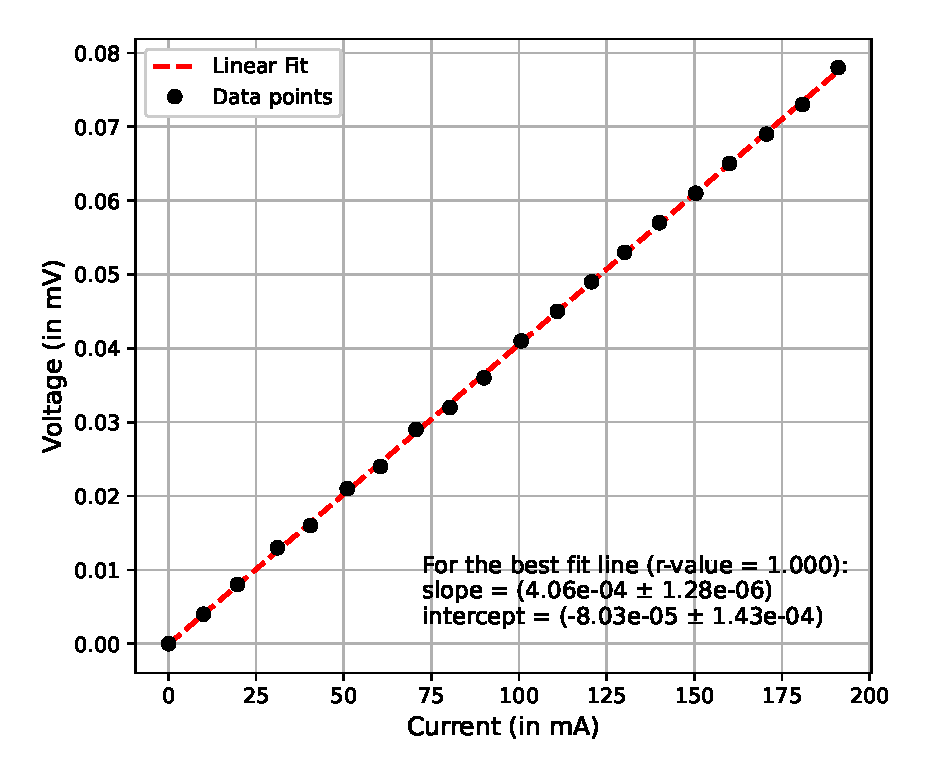
\includegraphics[width=1\columnwidth]{images/al.eps}
    \caption{V-I plot for the Aluminium sample at room temperature}
    \label{1}
\end{figure} 
Plugging the slope in Eq. 8, the resistivity at room temperature of Aluminium comes out to be $\rho = 3.131 \times 10^{-5}\,\,\Omega$ cm.
\vspace{-2em}
\subsubsection{n-Silicon}
The thickness of the provided sample was $W=(0.05 \pm 2\%)$ cm.
\begin{figure}[H]   
    \centering
    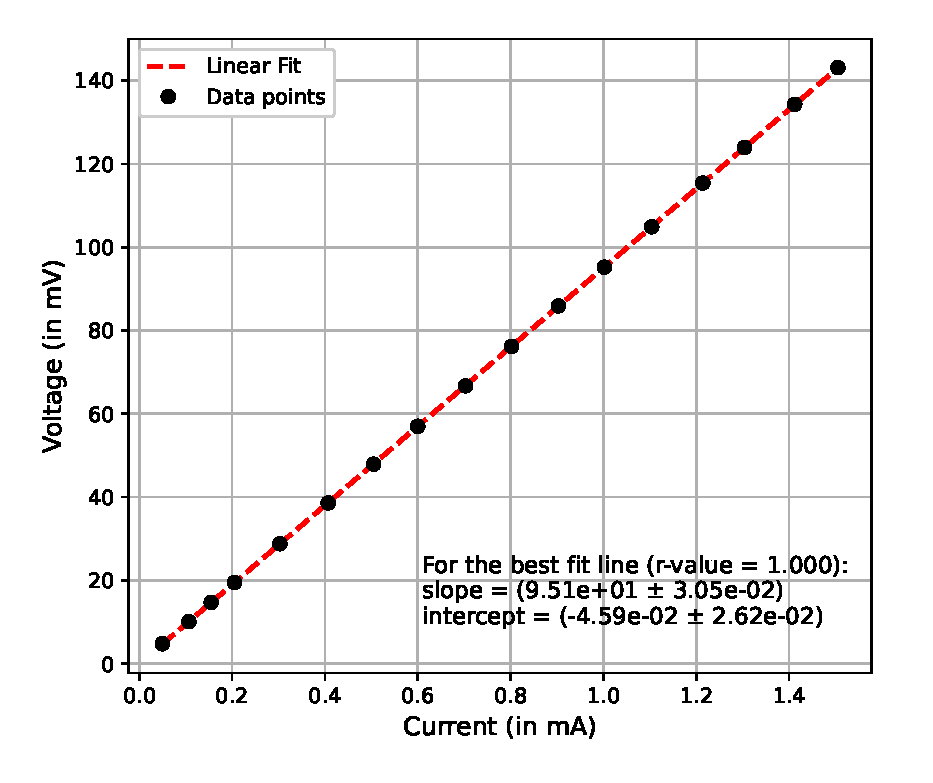
\includegraphics[width=1\columnwidth]{images/si.eps}
    \caption{V-I plot for n-Silicon at room temperature}
    \label{2}
\end{figure}
Plugging the slope in Eq. 8, the resistivity at room temperature of n-Si comes out to be $\rho = 21.549\,\,\Omega$ cm.
\vspace{-3em}
\subsubsection{n-Germanium}
\vspace{-2em}
\begin{figure}[H]   
    \centering
    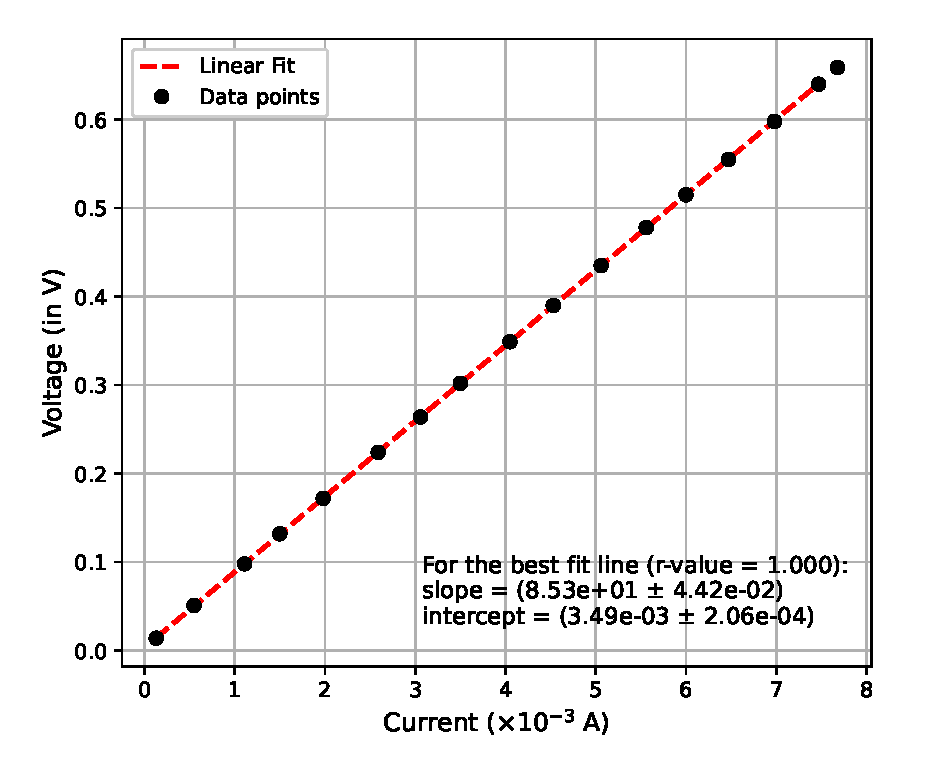
\includegraphics[width=1\columnwidth]{images/ge.eps}
    \caption{V-I plot for n-Germanium at room temperature}
    \label{3}
\end{figure}
Plugging the slope in Eq. 8, and using $W=(0.05 \pm 2\%)$ cm, the resistivity at room temperature of n-Ge comes out to be $\rho = 19.322\,\,\Omega$ cm.

\subsection{Estimation of Band-gap}
\subsubsection{n-Germanium}
\begin{table}[H]
\centering
\begin{tabular}{|c|c|c|} \hline
    $U$ (V)& $2r$ (cm) & $r$ (cm)  \\ \hline
    299.9 & 7.8 & 3.90  \\
    290.4 & 7.7 & 3.85 \\
    279.1 & 7.6 & 3.80 \\
    270.2 & 7.4 & 3.70  \\
    260.3 & 7.3 & 3.65 \\
    250.7 & 7.0 & 3.50  \\
    240.5 & 6.8 & 3.40  \\
    230.6 & 6.7 & 3.35 \\
    219.9 & 6.5 & 3.25 \\
    210.8 & 6.4 & 3.20  \\
    200.2 & 6.3 & 3.15 \\
    \hline
    \end{tabular}    
    \caption{$U$ vs $r$ data for a fixed $I=2$ A}
    \label{tab:3}
\end{table}
Table 2 shows the observed $T$-$V$ data. The error-bars are calculated with standard error propagation formulae (Section IV).
\begin{figure}[H]   
    \centering
    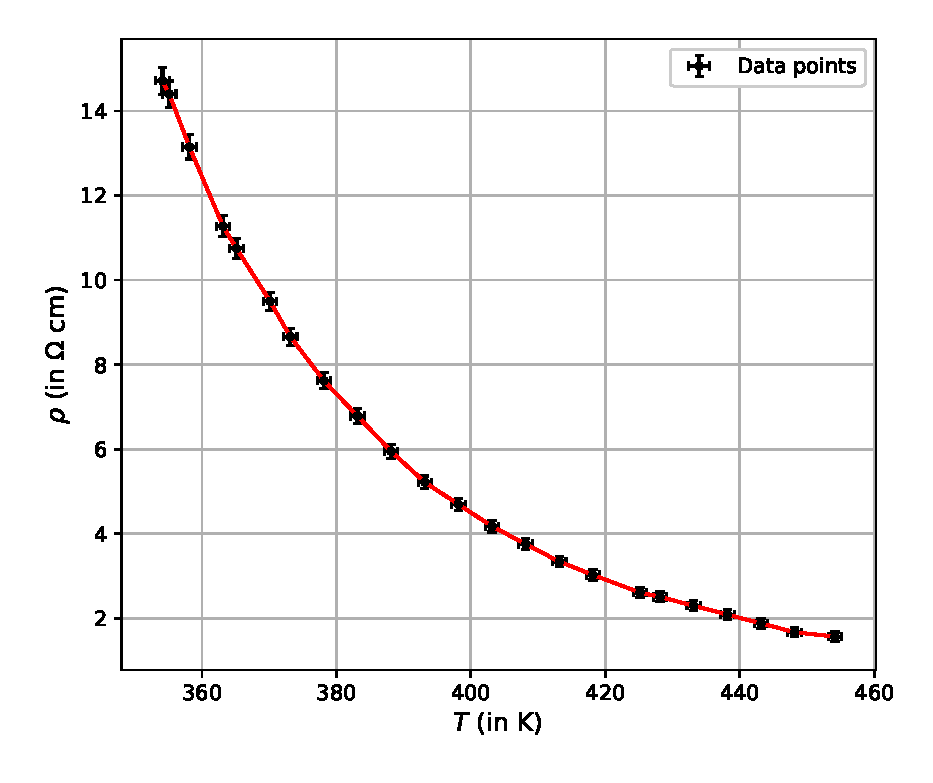
\includegraphics[width=1\columnwidth]{images/rho-ge.eps}
    \caption{$\rho$ vs. $T$ plot for n-Germanium for temperatures from 80$^\circ$C to 180$^\circ$C}
    \label{4.1}
\end{figure}
\begin{figure}[H]   
    \centering
    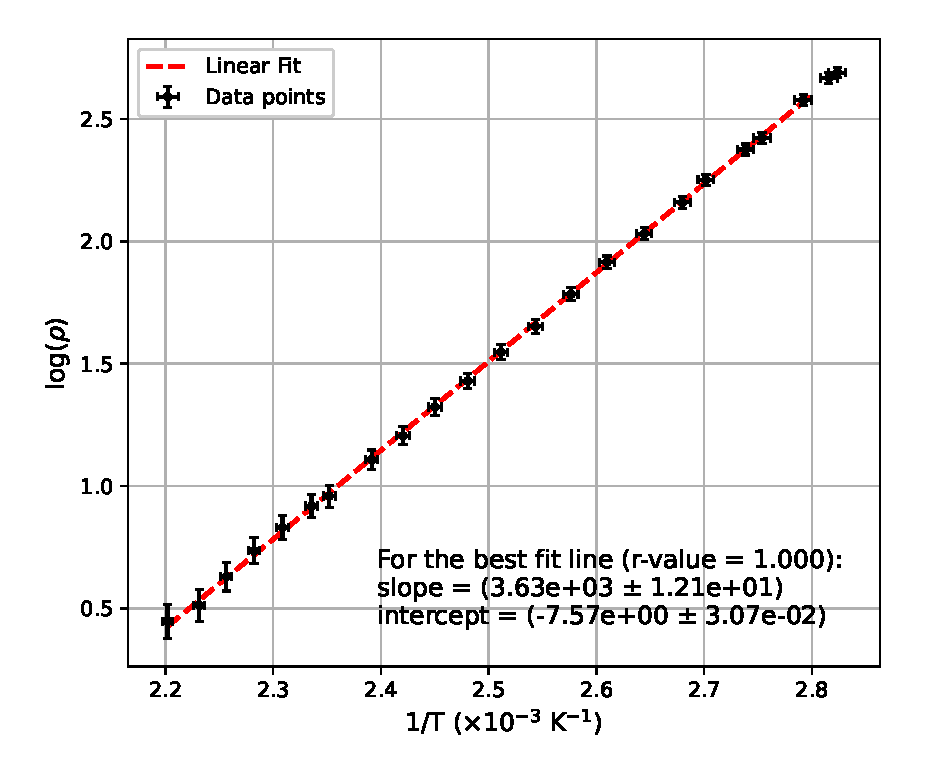
\includegraphics[width=1\columnwidth]{images/temp-ge.eps}
    \caption{$\log(\rho)$ vs. $T^{-1}$ plot for n-Germanium for temperatures from 80$^\circ$C to 180$^\circ$C}
    \label{4}
\end{figure}

From Fig. \ref{4}, we get the slope of $\log(\rho)$ vs. $T^{-1}$ which we can substitute into Eq. 9 to get the band-gap of the given Ge sample as,

\begin{align*}
    E_g = 2k_B\frac{\log(\rho)}{1/T} = 0.626 \text{ eV}
\end{align*}

\noindent where $k_B$ is the Boltzmann’s constant $= 8.6\times 10^{-5}$ eV/K.
\subsubsection{Aluminium}
Table 3 shows the observed $T$-$V$ data.
\begin{table}[H]
    \centering
    \begin{tabular}{|c|c|c|}
    \hline
    $T$ (in $^\circ$C) & $V$ (mV) & $\rho$ ($\times 10^{-5}\,\Omega$ cm) \\ \hline
    32 & 0.044 & 7.806 \\ 
    40 & 0.045 & 7.984 \\ 
    43 & 0.046 & 8.161 \\ 
    46 & 0.047 & 8.338 \\ 
    49 & 0.050 & 8.871 \\ 
    64 & 0.055 & 9.758 \\ 
    67 & 0.057 & 10.113 \\ 
    74 & 0.059 & 10.467 \\ 
    75 & 0.060 & 10.645 \\ 
    78 & 0.061 & 10.822 \\ 
    84 & 0.062 & 11.000 \\ 
    89 & 0.063 & 11.177 \\ 
    90 & 0.064 & 11.355 \\ \hline
    \end{tabular}
    \caption{Temperature dependence of $V$ and subsequently $\rho$ of the Al sample at a fixed $I=100$ mA.}
\label{tab:2}
\end{table}
\begin{figure}[H]   
    \centering
    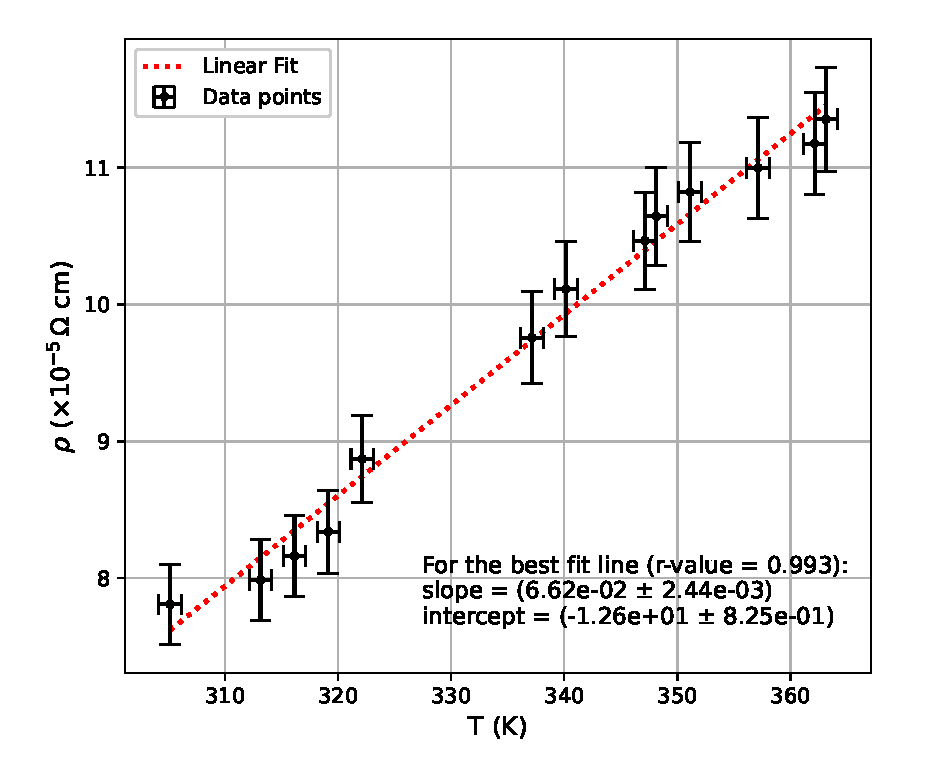
\includegraphics[width=1\columnwidth]{images/temp-al.eps}
    \caption{$\rho$ vs. $T$ plot for the Aluminium sample for temperatures from 32$^\circ$C to 90$^\circ$C}
    \label{5}
\end{figure}
For the temperature range used in this experiment (around 30$^\circ$C to 90$^\circ$C), we can theory predicts that the rise in $\rho$ with temperature is is roughly of linear order. Using, the linear relation,

\begin{align}
    \rho &= \rho_{T_0}[1+\alpha (T-T_0)]\\
    \text{or, }\rho &= \rho_{T_0} \alpha T + \rho_{T_0}(1-\alpha T_0) \nonumber 
\end{align}

\noindent and the linear fit in Fig. \ref{5}, we can approximate the temperature coefficient, $\alpha$ to be,

\begin{align*}
    \alpha = \frac{\text{slope}}{\rho_{T_0}} = 8.475 \times 10^{-3} \text{ K}^{-1}
\end{align*}

\noindent where $T_0=32^\circ$C $=304.15$ K.

\section{Error Analysis}
The error in the resistivity comes from the error of the slope of the fitted curve and the uncertainities in the thickness of the sample.

\begin{align}
    \frac{\Delta \rho}{\rho} = \sqrt{\left(\frac{\Delta W}{W}\right)^2 + \left(\frac{\Delta \text{slope}}{\text{slope}}\right)^2}
\end{align}

For the Al sample, $\Delta W = 0.001$ cm and for n-Si and n-Ge, $\Delta W/W = 2\%$. Plugging in $\Delta \text{slope}$ from Figs. \ref{1} to \ref{3}, we get

\begin{itemize}
    \item $(\Delta \rho)_\text{Al} = (0.184 \times 10^{-5})\,\,\Omega$ cm 
    \item $(\Delta \rho)_\text{n-Ge} = 0.387\,\,\Omega$ cm 
    \item $(\Delta \rho)_\text{n-Si} = 0.431\,\,\Omega$ cm 
\end{itemize}

\noindent For the uncertainity in $E_g$, we can similarly write,
\begin{align}
    \Delta E_g = E_g\left(\frac{\Delta \text{slope}}{\text{slope}}\right)
\end{align}

\noindent where the slope is the slope in the linear fit of the $\log(\rho)$ vs. $T^{-1}$ plot. Plugging in the values, we get for the n-Ge sample, $\Delta E_g=0.002$ eV.

The error in the temperature coefficient, $\alpha$ can similarly be derived using,

\begin{align}
    \frac{\Delta \alpha}{\alpha} = \sqrt{\left(\frac{\Delta \rho_{T_0}}{\rho_{T_0}}\right)^2 + \left(\frac{\Delta \text{slope}}{\text{slope}}\right)^2}
\end{align}

\noindent Using Table 3 and putting $\Delta \rho_{T_0}=0.290\,\Omega$ cm, we get $\Delta \alpha = 0.442$ K$^{-1}$.

